\documentclass[a4paper,11pt]{article}
\usepackage[utf8]{inputenc}
\usepackage{amsmath}
\usepackage{amsfonts}
\usepackage{amssymb}
\usepackage{graphicx}
\usepackage[backend=biber]{biblatex}

\addbibresource{nn.bib}
\renewcommand\thesubsection{\alph{subsection}}


%opening
\title{Computational properties of neural microcolumns arising from temporal dynamics}
\author{Vince Baker, advisor: Dr. Luis Cruz Cruz\\ Drexel University Department of Physics}

\begin{document}

\maketitle

\begin{abstract}
 The human brain hosts advanced cognitive processes that remain only partially understood.
Computational neuroscience seeks to understand brain functions through modeling at several levels of physical fidelity.
``Biologically inspired'' computation models are used in machine learning to solve a variety of problems that are intractable with conventional approaches.
Computational biophysics provides insight into the lowest levels of neural functions while nonlinear dynamics provides tools for understanding some aspects of cognition.
This research will explore the computational properties of neural networks through a novel combination of biophysics, nonlinear dynamics and machine learning.
\end{abstract}

\section{Introduction} 
There is no universal method to quantify the processing capability of a neural network.
In the machine learning community network models are developed and trained to solve specific problems, with the trained networks then graded against data sets representing those specific problems.
These computational network models include multi-layer perceptrons [ref], feed-forward "convolutional" networks [ref], and recurrent networks with memory [ref].
These models have been effectively applied to solve diverse problems including image recognition and classification, speech recognition and handwriting recognition.
The common computational models may be considered biologically-inspired, but none of them are biologically plausible.
All of these approaches greatly simplify the network and synapse dynamics.
Multi-layer perceptrons and feed-forward networks do not include recurrent connections, and are trained through biologically unrealistic methods involving back-propagation of error terms.
Recurrent network models such as long short-term memory (LSTM) [ref] incorporate feedback with a basic concept of memory, but the dynamics and training mechanisms are still not biologically plausible. \\
In this work we adapt the more biologically plausible Liquid State Machine (LSM) model first developed in \cite{maas2002}.
In the LSM model an untrained recurrent network, called the liquid or the reservoir, is excited with a time-varying input.
The stimulus perturbs the liquid and creates a complex state progression like pebbles dropped into a pond.
The time history of the input is encoded into the liquid state through the recurrent connections.
A trained readout network then decodes the desired information from the liquid state. \\
The LSM model is biologically plausible. 
The large liquid network can be randomly connected and is not trained.
The readout network can be trained with biologically plausible Hebbian learning and does not require error backpropagation.
Multiple readout networks can be trained to simultaneously extract different information from the same liquid network.
Liquid state machines have also proven an effective computational model, acheiving world-class results in speech recognition \cite{zhang2015}.
\\ \\
Discussion of approximation property, separation property, and fading memory.
\\
\begin{figure}[ht]
 \caption{Dynamic synapse models allow the LSM to recognize past inputs using the present state of the liquid \cite{maas2002}}
 \centering
   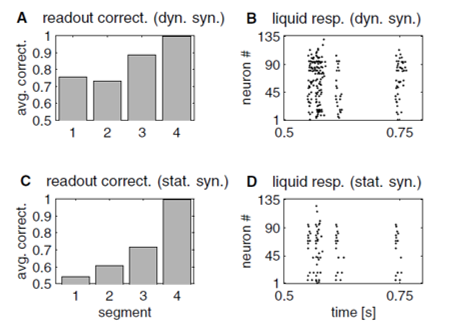
\includegraphics[width=\textwidth]{fig/maas_memory}
\end{figure}\\
\\ \\
To characterize the separation property of their liquid network Maas and Markram injected various spike trains and observed the resulting liquid states.
They defined the distance between two spike trains by correlating the spike trains against each other.
This definition is valid for closely related spike trains that may only differ by a translation in time.  
Improved distance metrics have been developed that are timescale-independent and time-resolved including inter-spike interval (ISI) and SPIKE \cite{kreuz2012}.
The SPIKE metric in particular provides an improved time-resolved distance metric across time scales and time shifts.
Figure from \cite{kreuz2012} demonstrates the time-resolved SPIKE metric (green) tracking three EEG signals that become synchronized over time.
\begin{figure}[ht]
	\caption{SPIKE metric applied to EEG data from \cite{kreuz2012}}
	\centering
	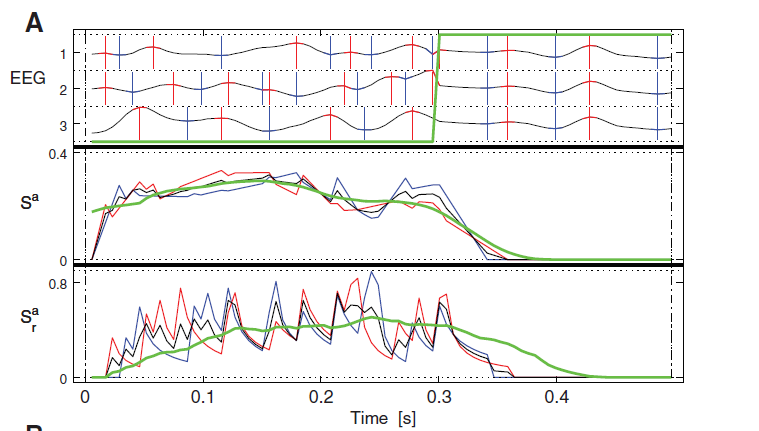
\includegraphics[width=\textwidth]{fig/SPIKE}
\end{figure}\\

\section{Methods}
Include graphic showing various neural models, highlight Izhikevich \cite{izhikevich2003} (MATLAB) and HH (NEURON) models for this work.
\begin{figure}[ht]
 \caption{Neural models}
 \centering
   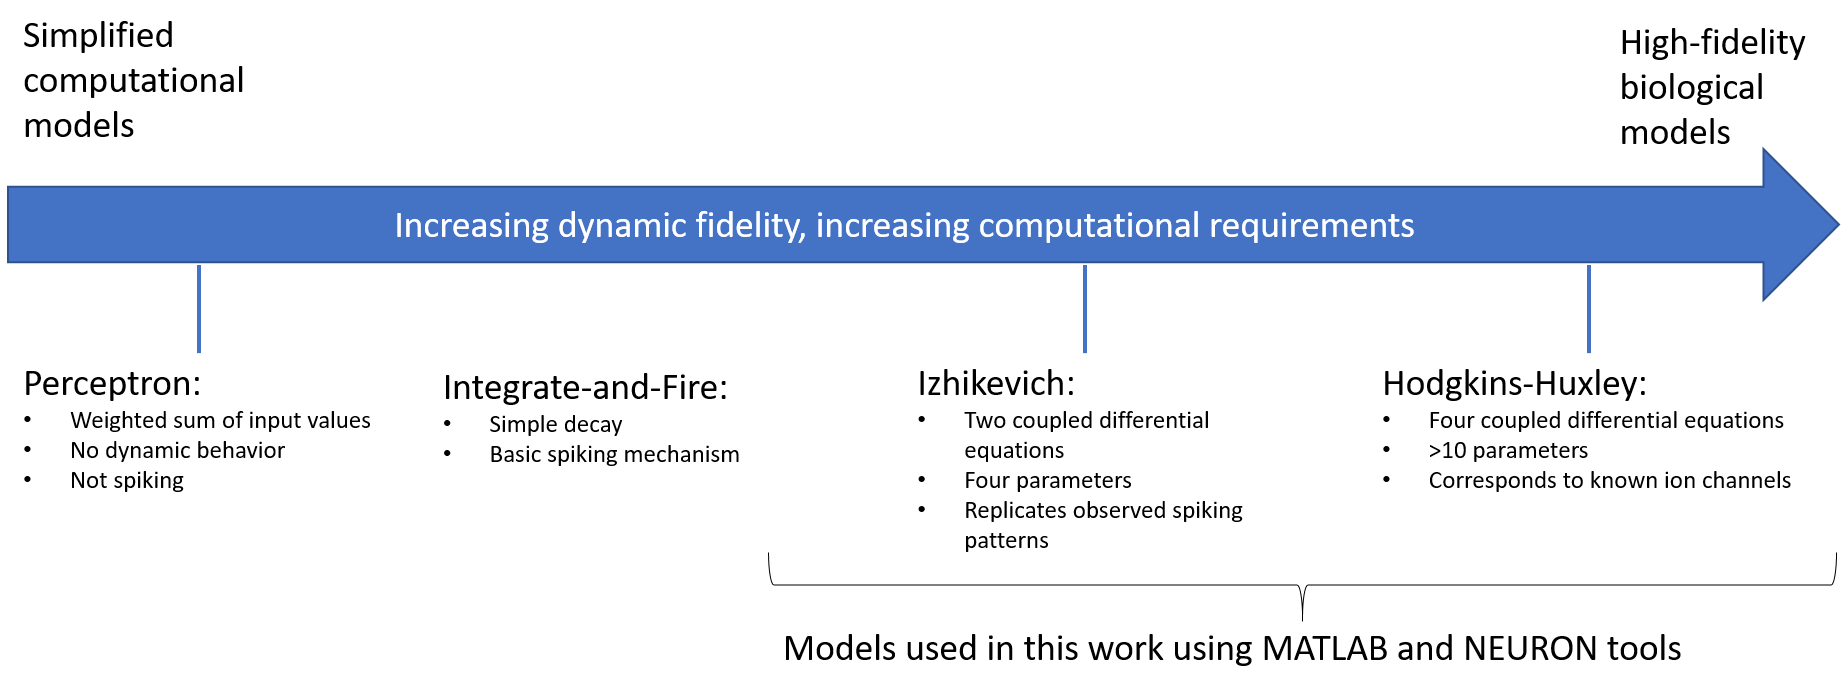
\includegraphics[width=\textwidth]{fig/neural_models}
\end{figure}\\
\\ \\
Our initial research re-examines the neural column circuit used as an LSM liquid network in \cite{maas2002}.
In their original work Maas and Markram used a simple integrate-and-fire neuron model combined with a sophisticted synapse model first presented in \cite{markram1998}.
The neural column was composed of 135 neurons on a unit column, 3x3 neurons wide and 9 neurons high.
The neurons were connected according to a distance-based rule $C \times e^{-(D(a,b)/\lambda)^2} $.
20\% of the neurons were inhibitory. 
The transmission delays between neurons were fixed to 1.5 ms for excitatory-excitatory connections and 0.8 ms for all other connections.
\\
In our initial research we have used a similar column structure and connectivity rule. 
Instead of I+F neurons we have chosen the Izhikevich model \cite{izhikevich2003} to allow us to explore the neural dynamics.
\\
\begin{figure}[ht]
 \caption{Column structure}
 \centering
   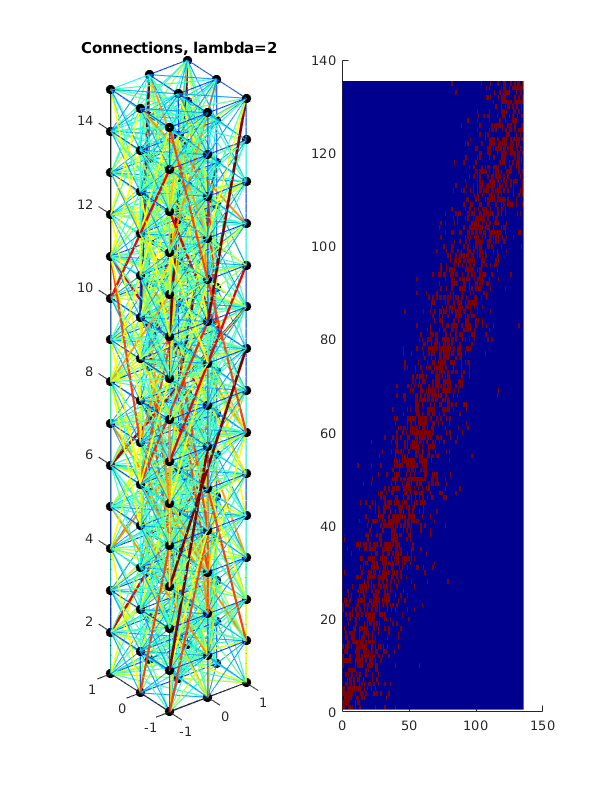
\includegraphics[width=200px]{fig/lambda2}
\end{figure}
\\
We enhanced the available MATLAB code for the Izhikevich model to incorporate propagation time between the neurons through the use of a delay buffer.
This allowed us to study the temporal effects of action potential propagation.
\\ \\
Introduce SPIKE metric and input/output distances-fading memory with association.
Compare to Maas Liquid State Machine measures of similarity.
\\ \\
\section{Results}
To test the effect of the distance-dependent propagation times we created two columns, 3x3x40,  with identical neurons and identical connectivity.
The first column has random propagation times, the second column has distance-dependent propagation times.
The bottom 10 layers were stimulated with random input as in \cite{izhikevich2003}.
The resulting firing patterns are shown below.
\\
\begin{figure}[ht]
 \caption{Column structure used in this research, $\lambda=2$,$C=1$,}
 \centering
   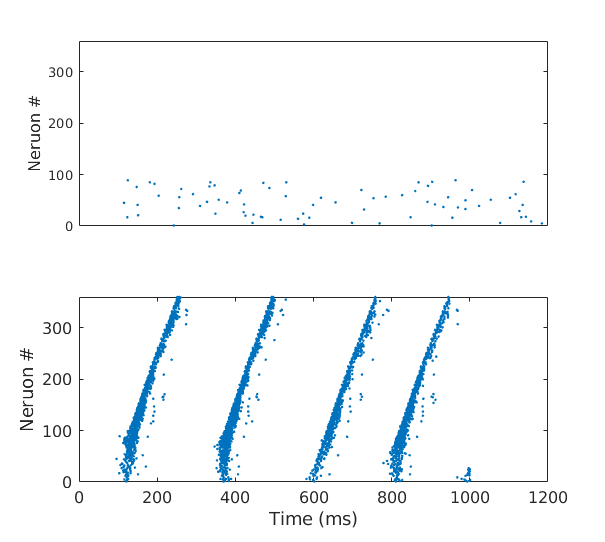
\includegraphics[width=\textwidth]{fig/DelayCompare_RandInput}
\end{figure}
\\
The column with random delay shows random firing activity in the stimulated region, but no propagation through the column.
The column with distance-dependent propagation shows correlated firings with a clear propagation down the column.
These results demonstrate that propagation delay is a critical parameter in the qualitative behavior of a neural column.
\\ \\
The current research, as well as previous research in our group [Tumulty ref], has found interesting behavior related to spike propagation time.
Biological spike velocity varies from about 1 meter/second for unmyelinated axons to >100 meters/second for myelinated axons.
On the millimeter and micrometer length scales of neural circuits this translates to propagation times orders of magnitude faster than neuron dynamic time scales.
There are several possible mechanisms through which slower effective propagation may occur.
Below we show that the spike propagation time is slower for narrower columns. 
This indicates a possible function of neural microcolumns, about 1 neuron wide, as slow-propagation channels in larger neural columns.
\\
\begin{figure}[ht]
 \caption{Effective propagation velocity}
 \centering
   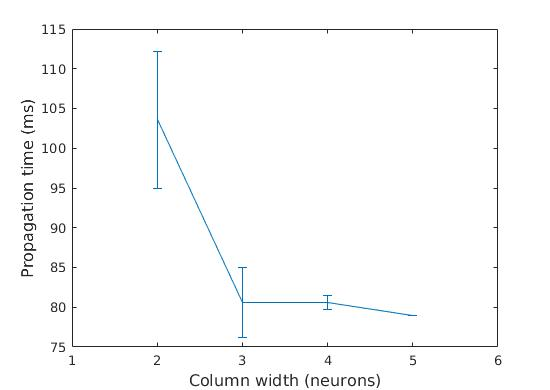
\includegraphics[width=\textwidth]{fig/propagation_time}
\end{figure}
\\ \\

\section{Future work}
Further investigation into mechanisms for lower effective velocity: spatial organization, neuron dynamics.\\
Neural dynamics near a bifurcation can result in a delayed firing \cite{izhikevich}.
Could be another mechanism for slower effective velocity.

\printbibliography

\end{document}
